\documentclass{standalone}
\usepackage{tikz}
\begin{document}
    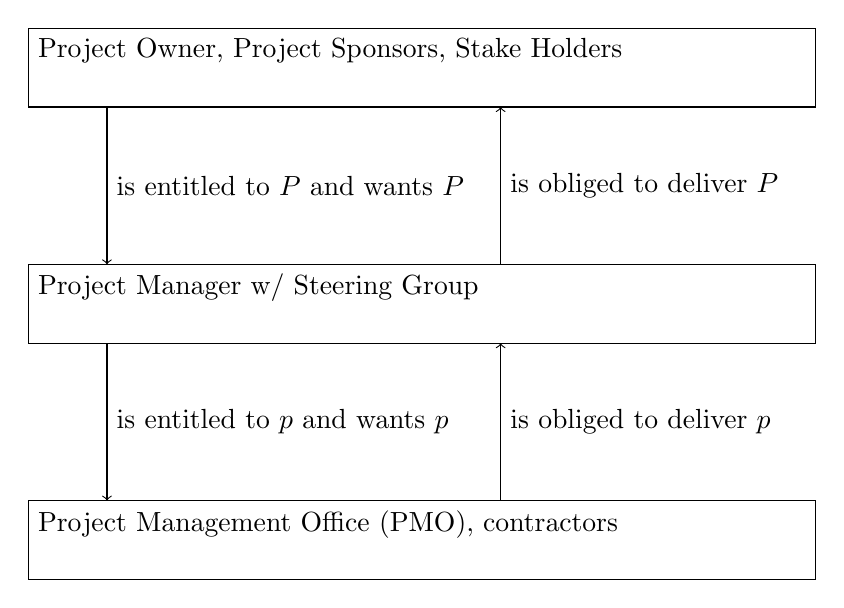
\begin{tikzpicture}
        \draw  (0,0) node[below right] {Project Owner, Project Sponsors, Stake Holders} rectangle (10,-1);
        
        \draw[->] (1,-1) -- node[right] {is entitled to $P$ and wants $P$} (1,-3);
        \draw[<-] (6,-1) -- node[right] {is obliged to deliver $P$} (6,-3);
        
        \draw  (0,-3) node[below right] {Project Manager w/ Steering Group} rectangle (10,-4);
        
        \draw[->] (1,-4) -- node[right] {is entitled to $p$ and wants $p$} (1,-6);
        \draw[<-] (6,-4) -- node[right] {is obliged to deliver $p$} (6,-6);
        
        \draw  (0,-6) node[below right] {Project Management Office (PMO), contractors} rectangle (10,-7);
    \end{tikzpicture}
\end{document}